%% rm report.pdf ; pdflatex -halt-on-error report.tex  && evince report.pdf
%% latex x.tex ; evince x.dvi

\documentclass[10pt,a4paper]{article}
% \documentclass[12pt]{report}
\usepackage{amsmath}

% gives us \url 
\usepackage{hyperref}

% indent the first para after a new section
%\usepackage{indentfirst}

% for png
\usepackage{graphicx}
\graphicspath{ {images/} }



% for figure captioning
%\usepackage[capposition=top]{floatrow}
%\usepackage{caption}
\usepackage{caption}

% to control positioning
\usepackage{float}

% missing - \usepackage{sectsty}


% control section fonts - it does work
\usepackage{sectsty}
\subsectionfont{\fontsize{10}{10}\selectfont}

% italic environment
\newenvironment{italicquotes}
{\begin{quote}\itshape}
{\end{quote}}

% bullet point lists
\let\Item\item
\newcommand\SpecialItem{\renewcommand\item[1][]{\Item[\textbullet~\bfseries##1]}}
\renewcommand\enddescription{\endlist\global\let\item\Item}

\title{Investigation into Control Vocabulary Publishing Services}
\date{}
\begin{document}
\SpecialItem

  \maketitle
    \begin{flushleft}


%  \setlength{\parindent}{5ex}

% 
% \section{High level requirements}
%   \item[Text] more text
%     and below
%   \item[and some] more text
%   \item[] empty
% \begin{italicquotes} hopefully italic  
%   and more italic
%   \end{italicquotes} 
% \url{http://www.uni.edu/~myname/best-website-ever.html}
% 

% need to be consisistent.


\section{
	Summary
}

\item[] IMOS/EMII should avoid pursuing their own ad-hoc solution and instead 
focus on integrating other provider's services and products to match needs due 
to limited development resources
\item[] LDP and SISSVoc are complementary solutions rather than alternatives
\item[] It's not self-evident that centralised registration management such as 
that provided by LDP necessarily matches IMOS/EMII organisational publishing 
requirements. Even LDP authors acknowledge their project is contrary to the 
non-federated nature of RDF publishing
\item[] Support for more sophisticated vocabulary authoring and development 
actions probably does not exist yet in the form of a web-based solution. For 
example, to support inferencing and consistency checking of OWL vocabularies already 
supported by dedicated third-party vocabulary applications, or to verify the 
reciprocal relationship of broader/narrower SKOS terms.
\item[] An investment has already been made around a controlled vocabulary 
database. This includes supporting the appending of Geoserver parameter and 
unit information at download and 
as a source of SKOS vocabulary for Geonetwork/Portal 123 for faceted search. 
Abandoning this effort would require the establishment of new work-flows
\item[] LDP is currently unfunded, lacking project oversight, technical 
support, points of contact or active discussion forums. It clearly presents an infeasible technical-risk 
unless there is a consensus from multiple external groups on new funding and 
feature development 


\clearpage

% multiple SISSVOC publishers have emerged and co-operate well together 

% have a section on background

\section{
  Tasks undertaken
}

%  
  The following tasks were completed:  

    \item[] A local instance of SISSVoc using preconfigured external SPARQL
  endpoints for various service providers was run-up under a tomcat webserver and
  demonstrated during Iteration review.  \footnote{ \url {
  http://github.com/jyucsiro/SISSVoc-runner }  } 

    \item[] It was found to be very difficult to glean an understanding of the
  functionality of LDP by reading source-code and internal development
  literature. Therefore a version of UKGovLD was also run-up on a private Nectar
  VM allocation. This followed prior unsuccessful attempts to provision a vagrant
  example of UKGovLD.  \footnote{ \url {
  https://github.com/UKGovLD/registry-deploy-poc } and \url {
  http://ukgovld-registry.s3.amazonaws.com/distribution/ukl-registry-0.0.1-SNAPSHOT-dist.tar.gz
  } }
  %
    Attempting to generate a dummy configuration for LDP and login with
  administrative privileges was fruitless, due to a bug in open-id redirection.
  However it was possible to explore and navigate the main menu-system of the
  application.
  %
    The discussion of LDP features is therefore more limited.

    \item[] Preliminary scripts to extract and encode the contents of the IMOS
  controlled vocabulary database as SKOS were written to guage the difficulty to
  perform the required mapping. These were further modified to be suitable to
  input into Geonetwork for current development to support platform / parameter
  based faceted search. Such export feature would probably also be necessary for
  upload to a publishing provider eg. ANDS or purl.org. 

    \item[] Attempted to register with ANDS and obtain an account to establish a
  test registry of published vocabulary terms. There were some technical issues,
  requiring help from ANDS technical support which were unresolved.
      
    \item[] SISSVoc and LDP was assesed against the \textit{High Level Functional
  Requirements For Vocabulary and Term Publishing} previously prepared by Project
  Officers.
    

\clearpage


\section { 
	High Level Functional Requirements For Vocabulary and Term Publishing
}

% OK
% 1 
  \subsection{
   Main function is to provide a resolvable endpoint for a vocabulary and its
  included terms (and details) using persistent identifiers.* 
  }

  \item For each term in the vocabulary persistent identifiers {URI} should
  be de-referenceable to the RDF item description. 

  \item SISSVoc as a standalone application has no inherent support for managing persistent
  identifiers. The main SISSVoc paper describes a deployment \footnote{ See Figure 3,
  SISSVoc: A Linked Data API for SKOS vocabularies.

  \url{http://www.semantic-web-journal.net/system/files/swj658.pdf} }, using a
  Persistent Identifier Service to map persistent URI resources to SISSVoc
  webservice urls but doesn't give futher details on the implementation or
  whether an external provider was chosen. 

  \item ANDS controlled vocabulary services build upons SISSVoc, although it appears
  their persistent identifier service is a more general organisational capability. According to
  documentation ANDS has, 

  \begin{italicquotes} [...] a simple HTTP-based interface, [which] ensures that
  identifier services can be integrated easily into existing data management
  workflows.  \end{italicquotes}
  Futhermore, ANDS does undertake to persist the infrastructure required for
  keeping its identifiers online. Ideally this service would be integrated
  with other SISSVoc vocabulary management functionality, although this was not tested.

  \item[]Another alternative, would be to use a service such as \url{purl.org}  \footnote{ The most
  prominent instances of such schemes are PURLexternal link, which has been used
  by the National Library of Australia, and ARKexternal link, at the California
  Digital Library. 

  Purl provides high-level adminstrative functionality for managing Persistent Uniform Resource 
  Locators, including Users, Groups, Domains, Help etc.
 }. 

  \item[]It would probably also be simple a step to publish identifiers under using an
  AODN or EMII dns based url. In this context, seegrid appear to have developed their own
  PID service used in conjunction with their own SISSVoc deployment  \footnote{
  https://www.seegrid.csiro.au/wiki/Siss/PIDService}  
  
  \item[]LDP is a resource registry management system, however it's unknown 
  if this includes direct support for persisent identifiers.
    \footnote{ See 
    https://github.com/UKGovLD/ukl-registry-poc/wiki/Principles-and-concepts
  }


% LDP -   The API should, where reasonable, follow REST principles. Specifically that
% any resource in the system should be identified by a URI and be manipulable by
% standard HTTP verbs (GET, PUT, DELETE, PATCH).
% 

% also supports versioning and management of PID could
%% ok, we got this restful stuff confused. GET,POST,DELETE,UPDATE... etc.
%% are html commANDS.

%   \# SISSVoc Deployment complemented by PID service
%   PURL. SISSVoc used a per
%   \url{https://www.seegrid.csiro.au/wiki/Siss/PIDService} 
% 
%   
%   SISSVoc - locally or externally hosted (ANDS) supports using persistent
%   identifiers.  Article tals branding. 4 things - expected.  Talk about rdf.
% 
%   SISSVoc is built upon rdf, and is a restful publishing api. 
%%   The DNS resolvable component of the uri, it is expected that ANDS will maintain
% 
%   ANDS and IMOS has extensive experience in managing in chef the DNS component of
%   names. Alternatively ANDS
% 


%% OK
% 2
\subsection{Resolvable content should be structured (or at least be able to be queried)
  using an RDF/SKOS encoding model. Content may however be adorned by other
  languages/metadata models (e.g. RDFS, OWL, Dublin Core).* }

  \item SISSVoc provides a linked data API for publishing SKOS vocabularies. SKOS
  is a standard vocabulary for thesarui, classifications, taxonomies and
controlled vocabularies using RDF.

   \item  The SISSVoc web-service API supports URI patterns that are aligned with the SKOS
  vocabulary model. This includes access patterns for SKOS Concept,
  ConceptScheme and Collection. Further URI patterns are provided to discover
  broader and narrower terms in transitive and non-transitive forms and according
  to text based labels. 

   \item SKOS content can be decorated with other RDF based
  content and persisted to any underlying triple store independently of SISSVoc
  functionality. SISSVoc provides
  no direct support URI patterns for search and discovery of such content. As an
  alternative, a SPARQL interface does provide a
  query/search mechanism for non-SKOS content such as DC, RDFS or OWL classes. 

  \item It is believed that LDP has no specific API support for SKOS resources.

%    According to Cox, SKOS lacks the expresitivity of languages such as OWL.
%   However common metadata standards like Dublin Core are supported.
%     It is anticipated that SKOS can be decorated with any data/metadata that can
%   be encoded in RDF triples.
% 
%   Additionally the SKOS Extensions RDF Vocabulary are a set of terms extending
%   the SKOS Core vocabulary to support some common features of knowledge
%   organisation systems, especially thesauri. (link) The extensions would appear
%   to be designed to cover common needs for representing authoring and publishing.
% 
%   Resolvable content - can be extracted SKOS Concepts from the already developed
%   relational vocab database demonstrates another approach which can then be
%   ingested to a RDF persistence. An example script has been created to demonstate
%   the feasibility of this approach. Alternately a SPARQL interface to RDF could
%   be used over the , to form RDF/SKOS content.
% 

% 3 
% NOT QUITE RIGHT - adminstratively customisable.
  \subsection{
  It should be possible to access vocabularies and their terms via an 
  (administratively) customisable Web-client interface and service interfaces.* } 

    SISSVoc provides a capable Web-client interface for read-only access
  vocabularies and their terms.

    In contrast to search, naviation and discovery, SISSVoc as a standalone
  application has no direct support for the creation and update of vocabulary
  terms. This is inherent to SISSVoc design, as a lightweight web-api implemented
  over a read-only based SPARQL endpoint/interface.  

  %   the SISSVoc client interface supports customisation, image branding which
  %   can be achieved via changes to css and js configuration.  Examples are
  %   given in the source code.  \footnote {
  %   https://github.com/jyucsiro/SISSVoc-runner/tree/master/SISSVoc/resources }
  %    
    According to the ANDS handbook, ANDS provides web-based GUI support for
  editing SKOS but only at file level.  \footnote { See 3.4.3, Editing
  Vocabularies \url{ http://www.ANDS.org.au/support/vocab-help-guide.pdf } }

    Some support for web-based versioning and author management at the file level
  is also available. Permissions to make change are tied to authority roles.

    \footnote { There is a need to consider whether file level versioning and
  management is sufficiently fine-grained. Also how should this interact with
  existing registry management already used in IMOS \texttt{control\_vocab\_db}.
  }
    
  % this doesn't quite belong, 
    For complex vocabulary authoring needs, SISSVoc authors suggest using an
  external vocabulary editor to maintain content that can also ensure that
  consistency of relationships between resources is maintained (eg. for OWL). 

    \begin{italicquotes} Vocabulary content may be maintained using RDF editors
  (such as Protégé 4 or TopBraid Composer 5 ), which ensure consistency of
  relationships between resources is maintained, and then generate RDF documents
  to transfer vocabulary content from the maintenance to publication envi-
  ronment, as outlined above. If a web-based vocabu- lary maintenance environment
  is required, then tools like TopQuadrant’s Enterprise Vocabulary Net 6 , and
  the PoolParty Thesaurus Server 7 are available.  \end{italicquotes} 

    \footnote { 3.2. HTTP operations and REST behaviour,
  \url{http://www.semantic-web-journal.net/system/files/swj658.pdf} }


% this REPEATS/CONFLICTS with subsection 3
% 4
\subsection{ 
  4. Most users require read only access to content.* 
}
  SISSVoc provides an easy-to-use Web-client interface for read-only access vocabularies and their terms.

  In contrast to search, navigation and discovery, SISSVoc as a standalone application has no direct 
  support for the creation and update of vocabulary terms. This is inherent to SISSVoc design, as a 
  lightweight web-api implemented over a read-only SPARQL endpoint/interface.  

  ANDS extends SISSVoc cabpability by including support for uploading, and raw editing
  at file-level. 

  LDP provides a Web-client for fine grained registry management of term
resources. But note, this is a general capability lacking SKOS specific functionality.


% OK
% 5
\subsection{ 
  There should ideally be a service interface that is REST-based* and a SPARQL service end-point.
}

    SISSVoc is designed with a HTTP-based interface aligned with REST-based web
services. The URI patterns facilitate SKOS discovery and access. However,
SISSVoc is not a full RESTful API, as it does not support HTTP operations for
update and deletion of resources.
    
    LDP is designed with a view to RESTFUL management of registry resources.
\footnote { https://github.com/UKGovLD/ukl-registry-poc/wiki/Api } It should be
noted that references to SKOS in the discussion of the LDP api apply to
registrars, not SKOS content maintained by particular registrars.  


    SPARQL (Simple Protocol and RDF Query Language) is an RDF query language
able to preserve, retrieve and manipulate data in RDF format and is a W3c
standard.  SPARQL abstracts the encoding model (XML, … etc), and persistence
layer and is adapted to the non-relational / graph structure of RDF.

    The SISSVoc RESTFUL URI patterns correspond quite closely with specific SPARQL queries
which perform the substantial work. SISSVoc thus relies on a SPARQL endpoint as the
mechanism to access RDF providing a strong separation of concerns.

    It would be feasible to map the already IMOS developed
\texttt{control\_vocab\_db} to expose a SPARQL interface using a tool such as
r2rml \footnote{ \url{ http://www.w3.org/TR/r2rml/ } } .  The SPARQL interface
would thus provide the endpoint for SISSVoc and replace the need to manage an
additional persistence layer.

	At least in standalone hosting, SISSVoc has supporting client-side SPARQL forms, 
	and showing the current SPARQL query.

    It is expected that an external SISSVoc provider such as ANDS would be
unlikely to expose such low-level query capability.
   

% OK
% 6
\subsection{ The publishing and retrieval service should offer and receive
re-direction(s) so that vocabularies or terms hosted on different domains (under
differing content authorities) can still be accessed via the service (if
desired). * }

{
SISSVoc supports seamless and consistent GUI navigation between differing
SISSVoc instances hosted on different domains.
%
Alternatively, normal url de-referencing allows navigation to non-SISSVoc
vocabulary implementations based around normal rdf resource uris.
%
Interestingly, due to the nature of the decoupled end-point design, SISSVoc 
can be configured to use multiple SPARQL endpoint providers. This unifies access
to different vocabulary providers from the same SISSVoc instance. 

% H=HERE
\begin{figure}[H]
\centering
\caption{SISSVoc using multiple SISSVoc domains}
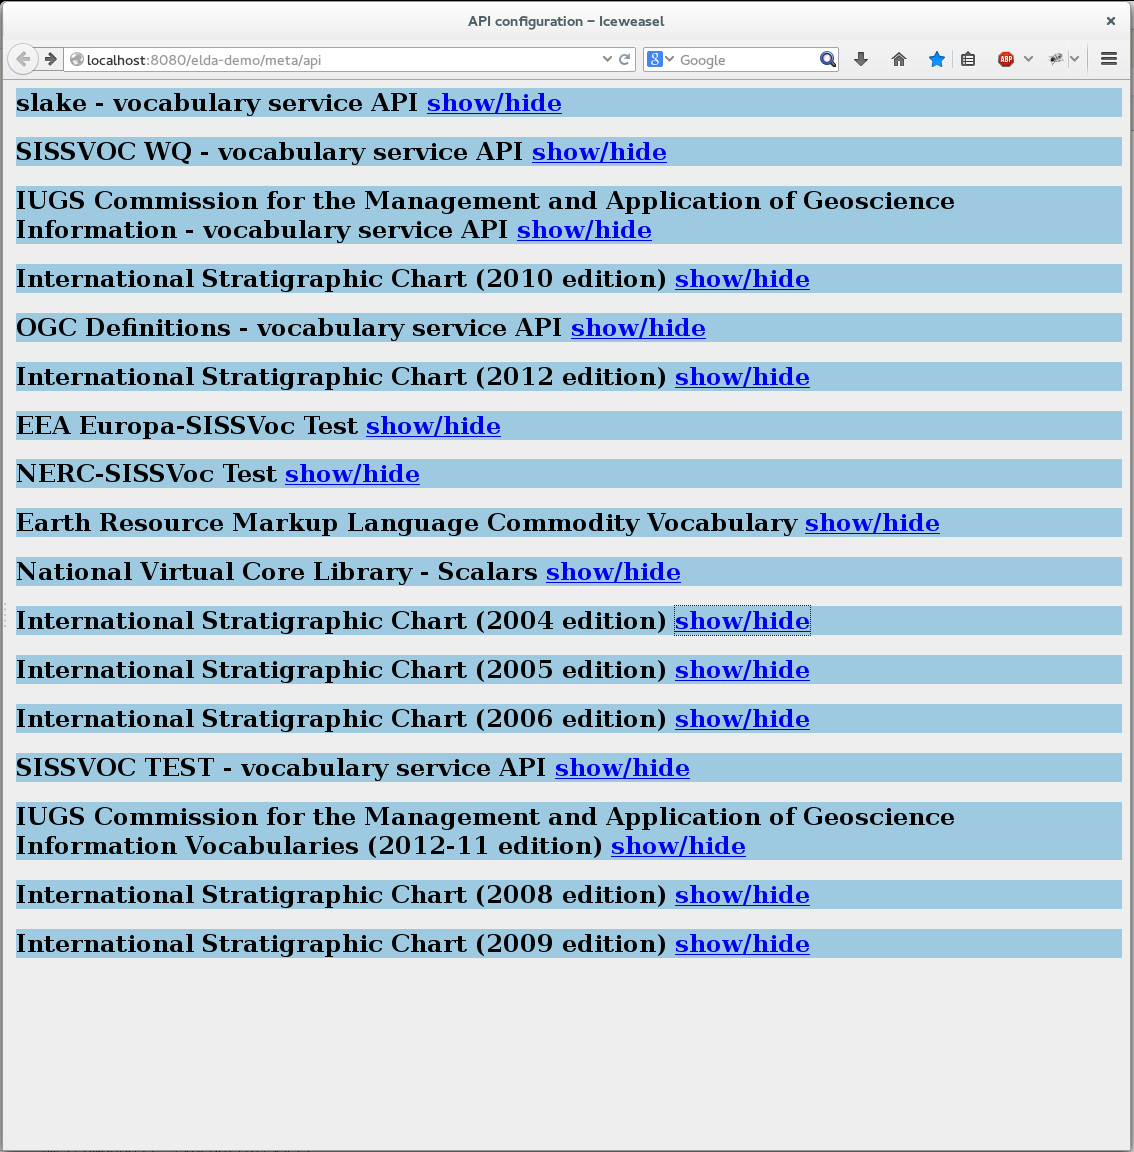
\includegraphics[width=12cm]{multipleendpoints}  
\label{fig:test}
\end{figure}

LDP GUI navigation capabilities are unknown, but assumed to be limited to 
registry management.
}
%
%
% CRAP 
%7
\subsection{ The Web-client should support some basic ‘canned’ querying (e.g.
free text search against concept, collection and scheme ‘labels’; traversing a
named vocabulary via hypertext links to explore included terms, their details
and any matches or mappings to other published vocabularies). * }
%
SISSVoc supports free-text searching against concept labels. It can list
concept, collection and concept schemes. SISSVoc can also traverse links 
for associated broader and narrower terms. 

\begin{figure}[H]
\centering
\caption{SISSVoc Gui Concept search and results}
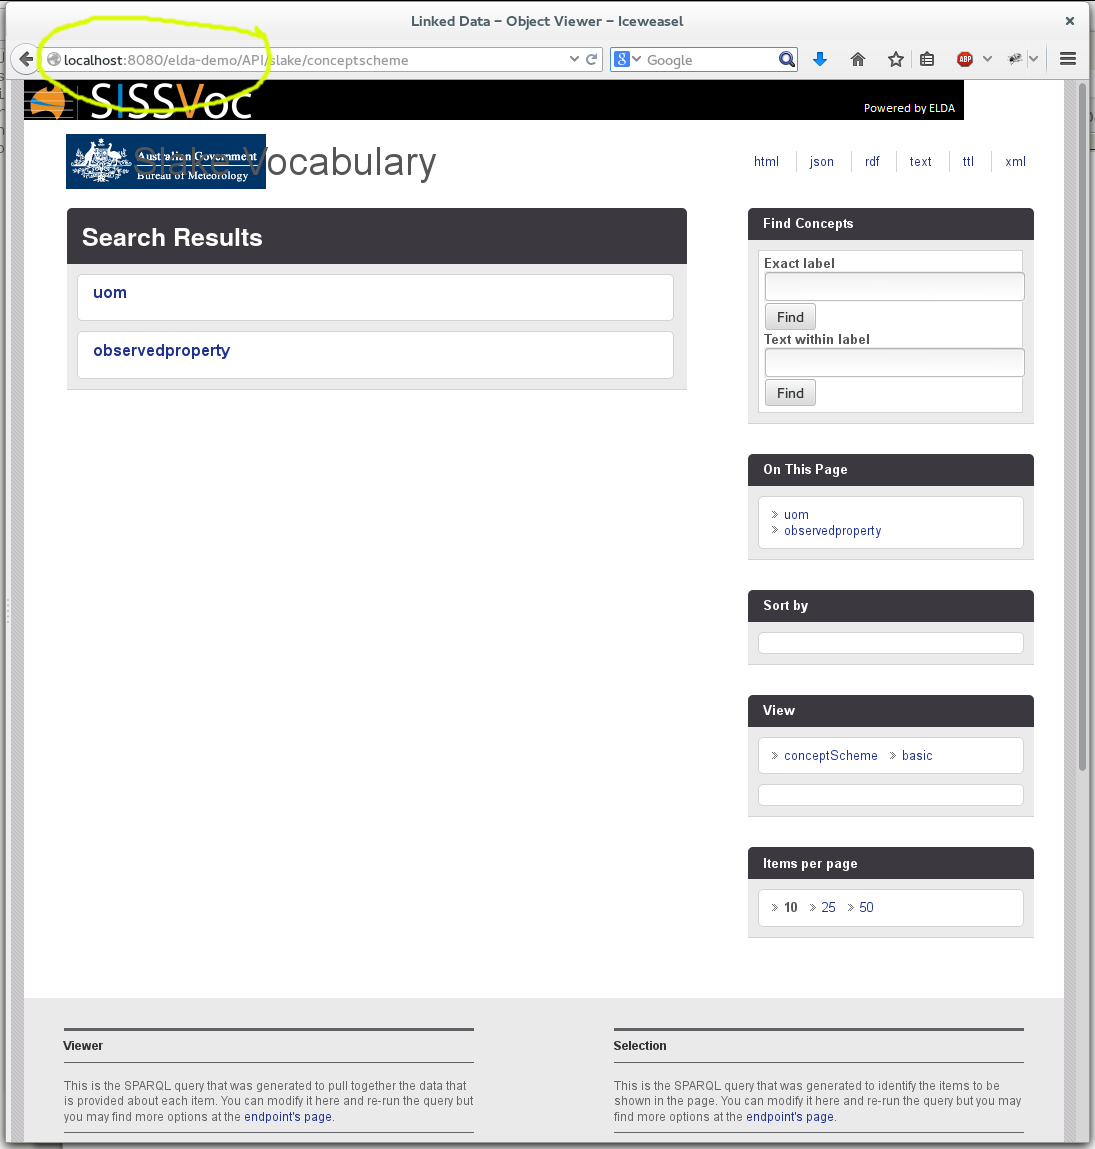
\includegraphics[width=12cm]{sissvoc}  
\label{fig:test}
\end{figure}



% SISSVoc - yes (local instance). configurable ttl - examples available.
% SISSVoc configuration is in RDF using TTL encoding. Lots of examples are given. 
% Need to assess - concept, collection, scheme each one individually.
% ANDS SISSVoc has also developed a vocabulary tree style widget
% https://researchdata.ANDS.org.au/developers/documentation/widgets/vocab_widget
% 

Support LDP capabilities for registrar searching are unknown.


% OK
% could include some screenshots of SISSVoc ?
% as an alternative protoge with a dedicated SKOS and OWL plugins. 
% 8
\subsection{ The Web-Client should be able to display in a user-friendly way
(e.g. using tables or forms) vocabulary and term details (e.g. scheme,
collection and concept labels; alt labels, its type, description, membership,
relations [including some Dublin core relations such as ‘publisher’ and ‘owner’
and revision info]). * }

The SISSVoc Web-Client supports user-friendly presentation of SKOS term details
including preferred label, definition, broader, and membership relations. Also
other metatadata terms such as Dublic Core source. 

It appears that the simple html table layout supports showing all associated rdf
properties if they are literals or rdfs:label types rather than URIs that
require dereferencing.

\begin{figure}[H]
\centering
\caption{SISSVoc Gui SKOS Resource }
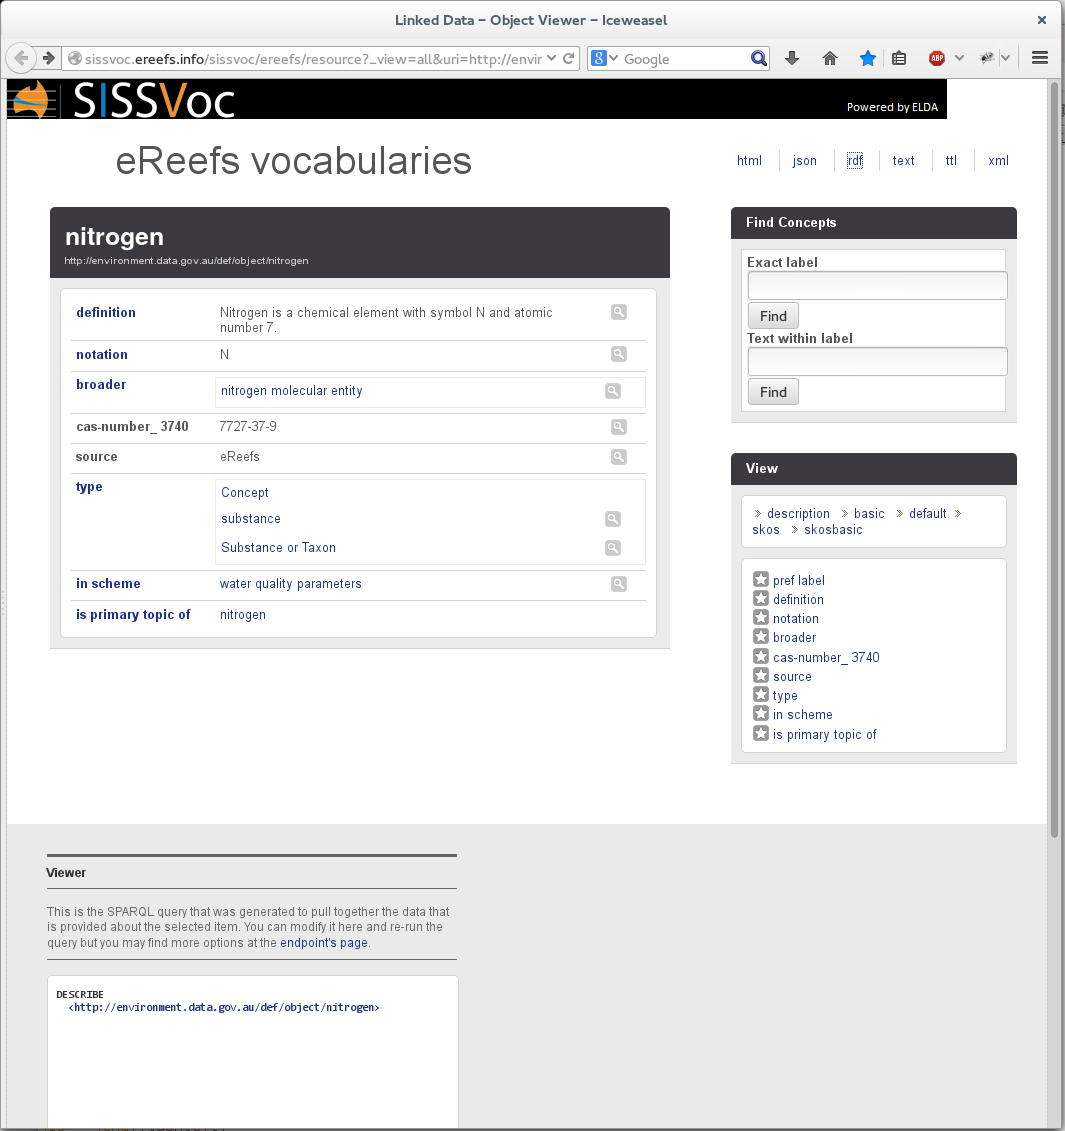
\includegraphics[width=12cm]{nitrogen}  
\label{fig:test}
\end{figure}


%%%%%%%%%%%%%%

% ALMOST OK.
%9 
\subsection{ 9. The Web-Client should be able to display categorized
(classified) lists of discoverable content (e.g. all vocabs by provided by
owner X; all terms in vocab Y) }

%owner - meaning - repo management.  classification - ?? must learn

\item[SISSVoc] as a stand-alone application has no notion of term ownership semantics.  
% importance of SKOS_XL Presumably  

\item [ANDS] may support since it combines registry management and SISSVoc. 

\item [LDP] may have support - unknown



% 10 
\subsection{ 10. The Web-Client should offer different formats in which to
download vocabularies or their terms (e.g. RDF*, text*, json, html*) }

SISSVoc supports downloading terms as html, json, rdf, text, ttl and xml. The
web-api has no support for downloading complete SKOS vocabularies except via a
manually crafted SPARQL request.

LDP's encoding support is unknown.

% ALMOST OK
% 11 
\subsection{ 11. The Web-Client should offer some statistics for users on the
type and volume of content available (e.g., number of vocabularies that can be
accessed and the number of terms in each vocabulary).  }
 

SISSVoc has no inherent support for compiling content statistics.

Using a SPARQL interface it ought to be trivial to construct queries to identy
for example the number of concepts, schemes, collections available with varying
search constraints applied. 

% ALMOST OK
% 12
\subsection{ 12. The publishing and retrieval service should be capable of
being configured to dynamically read one or more repository sources to access
content that needs to be published. * }

As has been described, a stand-alone SISSVoc test-runner can be configured to
read from multiple end-point sources. Although the front-end GUI support is not
very polished and uses different styling inconsistent with the rest of the
application.


% OK
% 13
\subsection{ 
13. Response times for retrieving queried content should be ‘user-tolerable’. *
}

During basic user-interface testing, both the local and remote \(ANDS\) options assume appear to be 
responsive. 

% It's expected that most of the speed will be backend / perssistence. 


% ROUGH
% 14
\subsection{  14. System should provide an administrative console/configuration
files to enable simple maintenance and administration (e.g., small changes to
Web-client interface displays and supported queries; to detect and fix broken
links in client-based hypertext; detecting missing details in retrieved content
– indicating content needs moderating/validating; provide basic statistics on
service usage).
}

Don't believe SISSVoc or LDP offer any administrative control over configuration. 

A locally deployed SISSVoc would permit the normal configuration possibilities that comes with controlling the
source code - css, ttl and javascript changes.

Usage statistics could be compiled using awstats, similar to other imos
web-apps. 

LDP usage 


\subsection{ 
15. There should be ‘meaningful’ error messaging provided in response to
service calls that cannot be satisfied (or which have been framed incorrectly).
* }

SISSVoc and LDP unknown 


%%% now need section on compiling and supporting. - mentioning the cost of deploying a web-app.  



\clearpage



end crap

  \end{flushleft}


  \textit{should be italic}


\LaTeX{} is a document preparation system for the \TeX{}
  typesetting program. It offers programmable desktop
  publishing features and extensive facilities for
  automating most aspects of typesetting and desktop
  publishing, including numbering and cross-referencing,
  tables and figures, page layout, bibliographies, and
  much more. \LaTeX{} was originally written in 1984 by
  Leslie Lamport and has become the dominant method for
  using \TeX; few people write in plain \TeX{} anymore.
  The current version is \LaTeXe.

  \begin{flushright}
  a para
  \textbf{should be bold}
  \textit{should be italic}

  \end{flushright}



  \begin{flushleft}
  My footnote\footnote{An example footnote.}
  Another footnote\footnote{Another footnote.}

  \hyperref[cnn]{http://www.cnn.com}

  \url{http://www.google.com}
  \href{http://www.google.com}{my google}
  \href{http://www.cnn.com}{http://www.cnn.com}

  % http://www.google.com
  \end{flushleft}
  more stuff
  more stuff2

  % This is a comment, not shown in final output.
  % The following shows typesetting power of LaTeX:
  \begin{align}
    E_0 &= mc^2                              \\
    E &= \frac{mc^2}{\sqrt{1-\frac{v^2}{c^2}}}
  \end{align}
\end{document}

